\chapter{Introducción}

Las \textbf{API} (en inglés “\textit{application programming interface}”) son hoy en día una parte fundamental de servicios y aplicaciones. Nos permite obtener datos, comunicar aplicaciones entre sí, y realizar una separación entre la parte lógica de la aplicación y la parte visual, pudiendo ser esta última una aplicación web, una de móvil, de televisión...

Es por eso que aprender y entender cómo crear una API es una parte fundamental que todo programador debe conocer, ya que de esta manera vamos a entender de mejor manera cómo funcionan. Esto nos será muy útil también, incluso, para utilizarlas.

Por todo ello, a continuación se va a explicar cómo hacer que nuestra aplicación cuente con API, para poder ser utilizada desde otra aplicación o para ser utilizada para obtener datos desde otro tipo de interfaz. Para ello, cabe recordar que las peticiones y los resultados deben ir en formato \href{https://es.wikipedia.org/wiki/JSON}{JSON}.


\chapter{Rutas para la API}

Hasta ahora hemos hecho uso del fichero \configfile{routes/web.php} para añadir rutas a nuestra aplicación. En el mismo directorio podemos ver que existe otro fichero llamado \configfile{routes/api.php}, que, como su propio nombre indica, vamos a utilizar para añadir las rutas que utilizaremos en nuestra API.

Si observamos el fichero, vemos ya existe una ruta creada:

\begin{mycode}{Contenido del fichero api.php}{php}{{\small }}
<?php
use Illuminate\Http\Request;
use Illuminate\Support\Facades\Route;

Route::middleware('auth:sanctum')->get('/user', function (Request $request) {
    return $request->user();
});
\end{mycode}

Si obtenemos el listado de rutas, veremos que ya existe una ruta para conocer el estado del usuario. A continuación vamos a añadir las rutas correspondientes para toda la gestión de los “posts” de nuestra aplicación.

Debemos recordar que para poder añadir las nuevas rutas, hay que incluir el controlador correspondiente, en este caso el \textbf{PostController}.

\begin{mycode}{Añadir nuevas rutas al fichero api.php}{php}{}
<?php
...
use App\Http\Controllers\PostController;
Route::resources([
    'posts' => PostController::class,
]);
\end{mycode}

Si ahora visualizamos el listado de rutas completo veremos las nuevas rutas. Si sólo nos interesan las rutas específicas a la API, podemos añadir un parámetro indicando sólo parte de la ruta, como se muestra a continuación:


\begin{mycode}{Añadir nuevas rutas al fichero web.php}{console}{{\small }}
root@5cff1feaf785:/var/www/html# php artisan route:list --path=api

GET|HEAD        api/posts ............ posts.index › PostController@index
POST            api/posts ............ posts.store › PostController@store
GET|HEAD        api/posts/create ..... posts.create › PostController@create
GET|HEAD        api/posts/{post} ..... posts.show › PostController@show
PUT|PATCH       api/posts/{post} ..... posts.update › PostController@update
DELETE          api/posts/{post} ..... posts.destroy › PostController@destroy
GET|HEAD        api/posts/{post}/edit  posts.edit › PostController@edit
GET|HEAD        api/user ....................................................
\end{mycode}

Por otro lado, dado que la API es un sistema en el que no vamos a guardar un estado (ya que haremos uso de \textit{\textbf{tokens}}), debemos hacer dos pequeños cambios a ficheros de configuración general.


En \configfile{app\Http\kernel.php} hay que modificar la sección de la API dejando:

\begin{mycode}{Modificar kernel.php}{php}{\small}
<?php
//...
'api' => [
    \Laravel\Sanctum\Http\Middleware\EnsureFrontendRequestsAreStateful::class,
    \Illuminate\Routing\Middleware\ThrottleRequests::class.':api',
    \Illuminate\Routing\Middleware\SubstituteBindings::class,
],
\end{mycode}

También hay que deshabilitar el \href{https://en.wikipedia.org/wiki/Cross-site\_request\_forgery}{CSRF} para estas rutas. Para ello modificamos el fichero \configfile{app\Http\Middleware\VerifyCsrfToken.php} dejando:

\begin{mycode}{Quitamos la protección CSRF a las rutas de la API}{php}{}
<?php
//...
    protected $except = [
        'api/*'
    ];
\end{mycode}

\chapter{Uso de controladores para la API}

Para que la modificación previa funcione es necesario modificar el controlador, ya que actualmente sólo devuelve la vista en formato código HTML. Por tanto, si queremos utilizar el mismo controlador, deberemos modificar las funciones. En el caso de la función “index” del PostController queda:


\begin{mycode}{Modificar la función de PostController}{php}{}
<?php
...
public function index(Request $request) {
    $posts = Post::orderBy('created_at')->get();
    if ($request->expectsJson()) {
        return response()->json($posts);
    } else {
        return view('posts.index',['posts' => $posts]);
    }
}
\end{mycode}

Tal como se puede ver, la función recibe dos modificaciones:

\begin{itemize}
    \item \textbf{Añadir parámetro “Request”}: De esta manera, podremos conocer si la petición viene desde la web, o si por el contrario se espera la respuesta en formato JSON.

    \item \textbf{Comprobar qué se espera}: Tal como se puede ver, se ha añadido un “if” donde se mira si la petición se espera en formato JSON (“expectsJson()”). En caso afirmativo, se devuelve la respuesta correspondiente en formato JSON.
\end{itemize}

\errorbox{\textbf{Es recomendable hacer uso de controladores específicos para la API}}



\section{Crear controladores específicos}

Debido a que las API se suelen versionar, es recomendable mantener los controladores de la web y de la API separados. Esto permite seguir el principio \textbf{\textit{KISS}} (\textit{Keep It Simple, Stupid!}). De esta manera se va a poder realizar modificaciones en un apartado de nuestra aplicación sin temer que podemos romper otra parte.

Es por ello, que lo ideal es crear controladores específicos para las funcionalidades que va a tener la API, y que se encuentren separados. Para ello realizaremos lo siguiente:

\begin{itemize}
    \item \textbf{Deshacer los cambios} de la función “index” vistos en el apartado anterior.
    \item \textbf{Crear nuevo controlador} que será específico para la API:

\begin{mycode}{Crear nuevo PostController exclusivo para la API}{console}{{\small}}
# php artisan make:controller API/PostController --api --model=Post
\end{mycode}

    Es necesario explicar lo siguiente:
    \begin{itemize}
        \item \textbf{“API/PostController”}: Esto indica cuál es la ruta donde se creará el fichero, que en este caso es \configfile{app/Http/Controllers/API/PostController.php}.

       \item \textbf{\texttt{--api}}: Este parámetro va a generar un controlador que carece de las funciones “create” y “edit”, ya que no son necesarias en una API, dado que son exclusivas a visualizar los formularios en un interfaz web.

       \item \textbf{\texttt{--model=Post}}: Para que el nuevo fichero del controlador ya tenga el include del modelo necesario.
    \end{itemize}

    \item \textbf{Modificar la ruta para la API} y que de esta manera haga uso del nuevo controlador exclusivo. El cambio es el siguiente:

\begin{mycode}{Modificar api.php para el nuevo controlador}{php}{}
<?php
...
use App\Http\Controllers\API\PostController;
\end{mycode}

    \item Modificar nuevo controlador, para que devuelva los datos correspondientes:

\begin{mycode}{Modificar el nuevo controlador PostController}{php}{}
<?php
...
use Illuminate\Http\Response;
public function index(){
    $posts = Post::orderBy('created_at')->get();
    return response()->json(['posts'=>$posts])
        ->setStatusCode(Response::HTTP_OK);
}
\end{mycode}

En este caso no hemos realizado ninguna comprobación, pero en una API de verdad debemos comprobar si se han encontrado resultados, y dependiendo de ellos devolver un \textbf{estado de respuesta distinto}.

La \href{https://github.com/symfony/symfony/blob/6.3/src/Symfony/Component/HttpFoundation/Response.php}{librería} contiene una gran cantidad de variables para hacer referencia a los posibles códigos que podemos devolver, así como el texto que acompañan al código.

\end{itemize}


\chapter{Comprobar funcionamiento}
Es momento de comprobar que todo funciona de manera correcta, y para ello debemos realizar una petición a la URL \href{http://localhost/api/posts}{http://localhost/api/posts} teniendo en cuenta el ejemplo que hemos estado realizando.

Para realizar la prueba podemos hacerlo de distintas formas, cada una de ellas dependiendo de la motivación que tengamos:

\begin{itemize}
    \item Utilizando un interfaz gráfico como \href{https://www.postman.com/}{Postman}, que nos va a facilitar hacer peticiones GET y peticiones más complejas.

    \begin{center}
        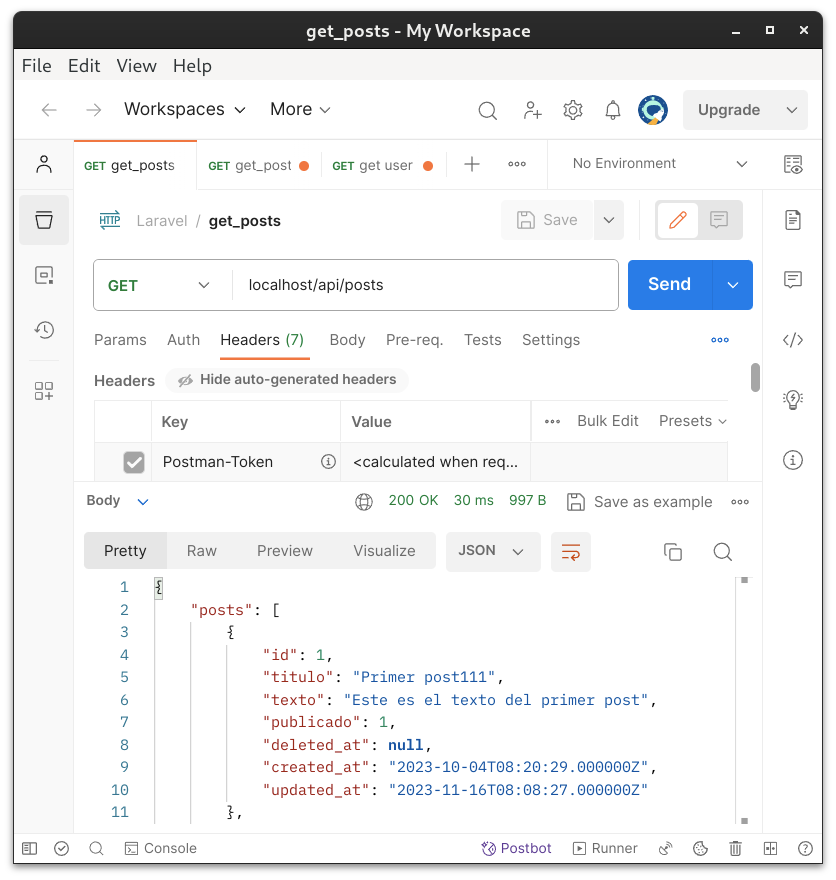
\includegraphics[width=0.7\linewidth]{postman.png}
    \end{center}

    \item Desde el propio \textbf{navegador web}. Veremos los datos JSON devueltos en formato texto directamente. Para comprobar que funciona, puede ser más que suficiente.




    \item Desde una \textbf{consola Linux}, haciendo uso del comando \textbf{curl}, podemos también comprobar de manera rápida si el \textit{endpoint} está funcionando:

\begin{mycode}{Modificar api.php para el nuevo controlador}{console}{}
ruben@vega:~$ curl -s  http://localhost/api/posts
{"posts":[{"id":1,"titulo":"Primer post111","texto":"Este es...”}]}
\end{mycode}

    Si queremos tener un resultado más visual, podremos hacer uso del comando “\textbf{jq}”, que deberemos instalarlo. De esta manera, podremos hacer:

\begin{mycode}{Modificar api.php para el nuevo controlador}{console}{}
ruben@vega:~$ curl -s  http://localhost/api/posts | jq
{
    "posts": [
      {
        "id": 1,
        "titulo": "Primer post111",
        "texto": "Este es el texto del primer post",
        "publicado": 1,
        "deleted_at": null,
        "created_at": "2023-10-04T08:20:29.000000Z",
        "updated_at": "2023-11-16T08:08:27.000000Z"
      }
    ]
}
\end{mycode}


\end{itemize}

\chapter{Autenticación}

Para poder realizar ciertas acciones a través de la API es lógico pensar que también deberemos estar autenticados, y para eso es necesario asegurar que al acceder a las rutas lo estemos. Para todo ello, vamos a crear un controlador propio donde tener en cuenta los datos que se envían al acceder a la API.

La idea general es que una aplicación al hacer uso de una API debe tener en cuenta:

\begin{itemize}
    \item Si el usuario no está registrado, poder registrarse.
    \item Si el usuario está registrado, se podrá loguear con lo que recibirá un \textbf{\textit{token}}.
    \item A partir de este momento, cada acción que quiera realizar, deberá ir acompañado del token para demostrar que está autenticado.
    \item Los \textit{tokens} pueden tener una vida útil. Por lo tanto, si el token expira, deberá volver a loguearse.
\end{itemize}

\section{Crear controlador de autenticación}

Se va a crear un controlador propio para tener el control de las acciones que se pueden realizar a través de la API, y así asegurar cuál es el estado de los tokens y/o del usuario que pide realizar una acción.

Para crear un controlador propio que sólo será usado para la API:

\begin{mycode}{Crear nuevo controlador}{console}{{\footnotesize }}
root@5cff1feaf785:/var/www/html# php artisan make:controller API/AuthController
INFO  Controller [app/Http/Controllers/API/AuthController.php] created successfully.
\end{mycode}

En este controlador vamos a tener tres funciones:

\begin{itemize}
    \item \textbf{register}: para que el usuario se pueda registrar.
    \item \textbf{login}: para que el usuario se pueda loguear y recibir un token.
    \item \textbf{logout}: para que el usuario se pueda desloguear y de esta manera el token se revoque.
\end{itemize}

El controlador, quedaría de la siguiente manera.

\errorbox{\textbf{Es importante entender qué hace cada una de las funciones}}

\begin{mycode}{Nuevo AuthController para la API}{php}{{\small }}
<?php
namespace App\Http\Controllers\API;
use App\Http\Controllers\Controller;
use Illuminate\Http\Request;

use App\Models\User;
use Illuminate\Support\Facades\Hash;
use Illuminate\Validation\ValidationException;
use Illuminate\Http\Response;

class AuthController extends Controller {

    public function register(Request $request){
        $validatedData = $request->validate([
        'name' => 'required|string|max:255',
        'email' => 'required|string|email|max:255|unique:users',
        'password' => 'required|string|min:8',
        ]);

        $user = User::create([
        'name' => $validatedData['name'],
        'email' => $validatedData['email'],
        'password' => Hash::make($validatedData['password']),
        ]);
        return response()->json([
        'name' => $user->name,
        'email' => $user->email,
        ])->setStatusCode(Response::HTTP_CREATED);
    }

    public function login(Request $request){
        $request->validate([
        'email' => 'required|email',
        'password' => 'required',
        'device_name' => 'required',
        ]);
        $user = User::where('email',  $request->email)->first();

        if (! $user || ! Hash::check($request->password, $user->password)){
            return response()->json([
            'message' => ['Username or password incorrect'],
            ])->setStatusCode(Response::HTTP_UNAUTHORIZED);
        }
        // FIXME: queremos dejar más dispositivos?
        // $user->tokens()->delete();

        return response()->json([
        'status' => 'success',
        'message' => 'User logged in successfully',
        'name' => $user->name,
        'token' => $user->createToken($request->device_name)
        ->plainTextToken,
        ]);
    }

    public function logout(Request $request){
        $request->user()->currentAccessToken()->delete();
        return response()->json([
        'status' => 'success',
        'message' => 'User logged out successfully'
        ])->setStatusCode(Response::HTTP_OK);
    }
}
\end{mycode}

Es importante notar un comentario que se ha dejado en la función “\textbf{login}”. Dependiendo de si queremos que la API permita tener varios tokens para un mismo usuario o no (posibles logins desde distintos dispositivos), deberemos dejar comentado o descomentar la línea indicada.

Para que estas funciones entren en juego, debemos modificar el fichero de rutas \configfile{api.php}

\begin{mycode}{Rutas de autenticación para la API}{php}{}
<?php
//...
Route::post('/register', [AuthController::class, 'register']);
Route::post('/login', [AuthController::class, 'login']);
Route::post('/logout', [AuthController::class, 'logout'])
    ->middleware('auth:sanctum');
\end{mycode}




\section{Modificar rutas}

Tal como hemos hecho anteriormente, para que la aplicación funcione bajo el sistema de autenticación, y que automáticamente nos indique que no estamos autenticados, debemos realizar la modificación del fichero de rutas \configfile{api.php}


De manera similar a la aplicación web, deberemos indicar qué rutas queremos que se puedan obtener sin estar autenticado y cuáles no.


\begin{mycode}{Rutas autenticadas para la API}{php}{}
<?php
//...
Route::middleware(['auth:sanctum'])->group(function () {
    Route::resources([
        'posts' => PostController::class,
    ]);
});

Route::controller(PostController::class)->group(function () {
    Route::get('/posts', 'index')->name('posts.index');
    Route::get('/posts/{post}', 'show')->name('posts.show');
})->withoutMiddleware(['auth:sanctum']);
\end{mycode}

\section{Pruebas de funcionamiento}


Para que la autenticación funcione, podemos realizar pruebas a través de Postman, de manera similar a como hemos hecho anteriormente. Ahora hay que tener en cuenta que la petición va a ser de tipo \textbf{POST}, y dado que queremos crear un \textit{post}, tendremos que realizar el paso de parámetros.

Por lo tanto, los pasos que debemos realizar son:

\begin{itemize}
    \item Realizar prueba de login. Debemos pasar los parámetros y obtendremos el token y una serie de datos extra, que podremos utilizar en nuestra aplicación.
    \begin{itemize}
        \item email
        \item password
        \item device\_name
    \end{itemize}

    \begin{center}
        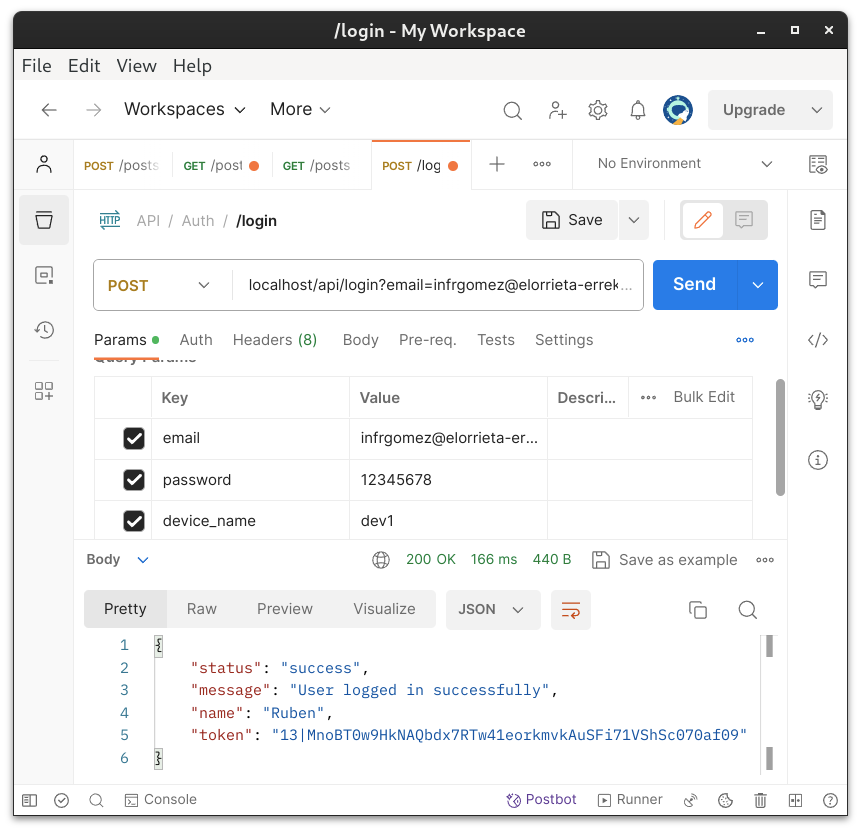
\includegraphics[width=0.8\linewidth]{postman_login.png}
    \end{center}

    \item Con ese token podremos realizar la prueba de añadir un nuevo \textit{post} a través de la API.

    \begin{center}
        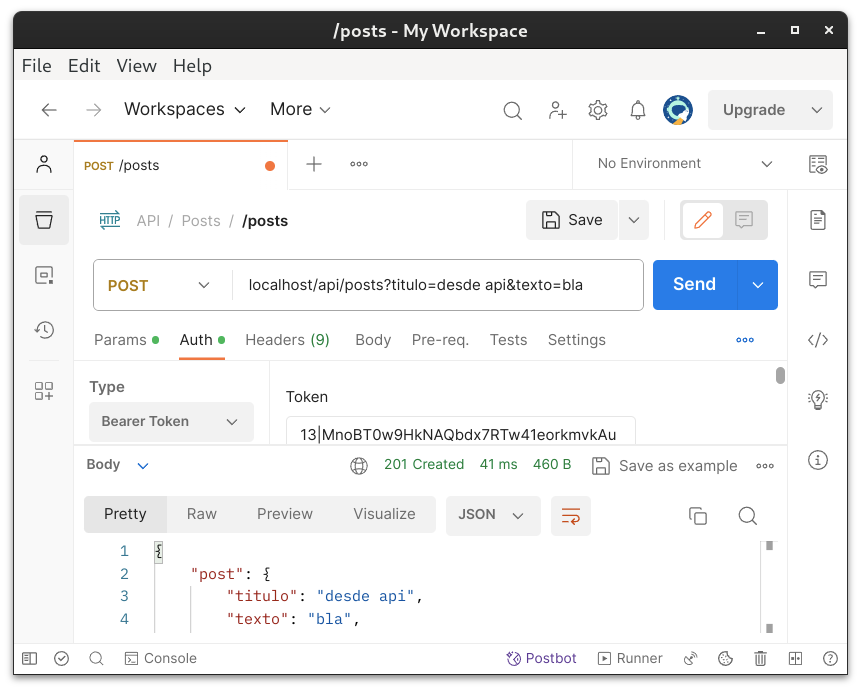
\includegraphics[width=0.8\linewidth]{postman_create.png}
    \end{center}

    Deberemos indicar:

    \begin{itemize}
        \item Los parámetros necesarios para la creación del \textit{post}: “título”, “texto” y “publicado”.
        \item El tipo de token de autenticación en la pestaña “Auth” de Postman tiene que ser de tipo “\textbf{Bearer Token}”.
    \end{itemize}

\end{itemize}


\chapter{Visualizar API}

Suele ser habitual tener un interfaz donde se muestra el funcionamiento de nuestra API, o cuáles son los \textit{endpoints} de la misma. Es decir, qué URL se pueden consultar, qué método hay que utilizar, si es necesario el paso de parámetros, ...

Hoy en día existe la especificación \href{https://www.openapis.org/}{OpenAPI} para la generación de la API, y sobre ella existen distintos interfaces web. Uno de los interfaces más utilizados es \href{https://swagger.io/tools/swagger-ui/}{Swagger UI} que nos muestra un bonito interfaz y a la vez es posible utilizarlo para realizar consultas a la API.

Para poder instalarlo en nuestro proyecto Laravel, necesitamos realizar la instalación de unas dependencias y la posterior instalación en el proyecto.

\begin{mycode}{Instalación de dependencias}{console}{{\small}}
root@5cff1feaf785:/var/www/html# composer require "darkaonline/l5-swagger"
root@5cff1feaf785:/var/www/html# php artisan vendor:publish \
    --provider "L5Swagger\L5SwaggerServiceProvider"
\end{mycode}


Para poder generar el interfaz de manera correcta añadimos comentarios a las funciones. En uno de los controladores añadiremos la siguiente cabecera, que nos va a servir para definir el tipo de autenticación:

\begin{mycode}{Cabecera para la API}{php}{}
<?php
//...
/**
* @OA\Info(title="API", version="1.0"),
* @OA\SecurityScheme(
*     in="header",
*     scheme="bearer",
*     bearerFormat="JWT",
*     securityScheme="bearerAuth",
*     type="http",
* ),
*/
\end{mycode}


Para documentar la función \textbf{index}, encima de ella añadiremos lo siguiente. Hay que darse cuenta que en este caso sólo hemos documentado la respuesta “200”.

\begin{mycode}{Comentario para /api/posts}{php}{}
<?php
//...
/**
* @OA\Get(
*     path="/api/posts",
*     summary="Mostrar posts",
*     @OA\Response(
*         response=200,
*         description="Mostrar todos los posts."
*     ),
*     @OA\Response(
*         response="default",
*         description="Ha ocurrido un error."
*     )
* )
*/
public function index(){
//...
\end{mycode}

Para documentar la función de guardar un \textit{post} desde la API, usaremos los siguientes comentarios:

\begin{mycode}{Comentario para función POST /api/posts}{php}{}
<?php
//...
    /**
* @OA\Post(
*     path="/api/posts",
*     summary="Create a post",
*     @OA\Parameter(
*         name="titulo",
*         in="query",
*         description="The title of the post",
*         required=true,
*         @OA\Schema(
*             type="string"
*         )
*     ),
*     @OA\Response(
*         response=200,
*         description="successful operation",
*         @OA\JsonContent(
*             type="string"
*         ),
*     ),
*     @OA\Response(
*         response=401,
*         description="Unauthenticated"
*     ),
*     security={
    *         {"bearerAuth": {}}
    *     }
* )
*/
public function store(Request $request){
\end{mycode}


Por último, vamos a poner otro ejemplo, para documentar el obtener un \textit{post} concreto. Para ello los comentarios serán:

\begin{mycode}{Comentario para /api/posts/{id}}{php}{}
<?php
//...
/**
* @OA\Get(
*     path="/api/posts/{id}",
*     summary="Mostrar un post concreto",
*     @OA\Parameter(
*          name="id",
*          description="Project id",
*          required=true,
*          in="path",
*          @OA\Schema(
*              type="integer"
*          )
*     ),
*     @OA\Response(
*         response=200,
*         description="Mostrar el post especificado."
*     ),
*     @OA\Response(
*         response="default",
*         description="Ha ocurrido un error."
*     )
* )
*/
public function show(Post $post){
\end{mycode}


Y para la función \textbf{show}, que sólo nos muestra un único post, añadiremos los siguientes comentarios:

\begin{mycode}{Comentario para /api/posts/ID}{php}{}
<?php
...
/**
* @OA\Get(
*     path="/api/posts/{id}",
*     summary="Mostrar un post concreto",
*     @OA\Parameter(
*          name="id",
*          description="Project id",
*          required=true,
*          in="path",
*          @OA\Schema(
*              type="integer"
*          )
*     ),
*     @OA\Response(
*         response=200,
*         description="Mostrar el post especificado."
*     ),
*     @OA\Response(
*         response="default",
*         description="Ha ocurrido un error."
*     )
* )
*/
public function show(Post $post) {
    //...
\end{mycode}


No se han añadido todos los parámetros en todos los casos, ya que resulta redundante y es fácil añadir los que faltan.

Para conocer todas las funcionalidades de los comentarios, es recomendable mirar la \href{https://github.com/zircote/swagger-php#usage}{documentación}. Desde aquí nos mostrará el enlace para la \href{https://zircote.github.io/swagger-php/#links}{documentación oficial de Swagger PHP}, o lo que nos puede resultar más interesante, que es un conjunto de \href{https://github.com/zircote/swagger-php/tree/master/Examples}{ejemplos} junto con el \href{https://petstore.swagger.io/#/}{resultado en forma de web}.


Tras esto, ejecutaremos el comando que recorrerá los controladores para generar el fichero \configfile{storage/api-docs/api-docs.json}. Este es el fichero que el interfaz web tendrá en cuenta a la hora de generar la web que podemos ver a continuación.

El comando es el siguiente:

\begin{mycode}{Generamos el fichero json para Swagger}{console}{}
root@5cff1feaf785:/var/www/html# php artisan l5-swagger:generate
Regenerating docs default
\end{mycode}



Tras ejecutar el comando anterior, si vamos a la url \href{http://localhost/api/documentation}{http://localhost/api/documentation} tendremos acceso y veremos el interfaz para nuestra API:

\begin{center}
    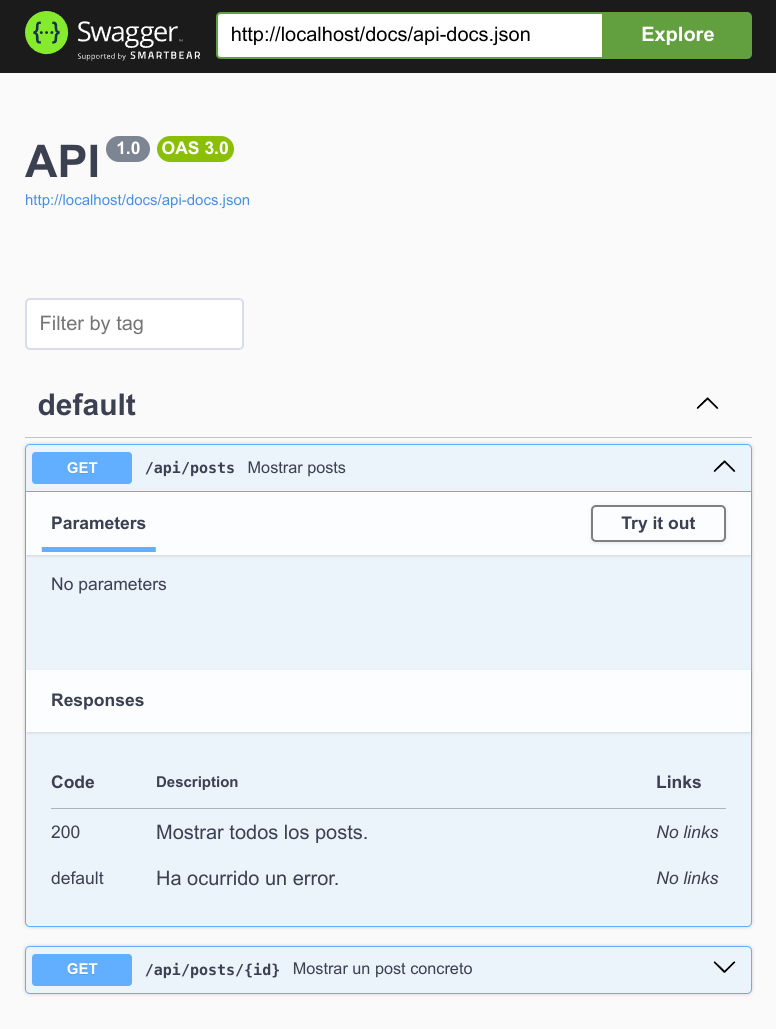
\includegraphics[frame,width=0.8\linewidth]{swagger.png}
\end{center}



\exercisebox{Completar los comentarios añadiendo los parámetros que faltan a la función de crear y los necesarios para la función de borrado de posts.}

% Mostrar SWAGGER.io
% https://styde.net/como-documentar-una-api-en-laravel-usando-swagger/
% https://github.com/DarkaOnLine/L5-Swagger
% https://github.com/zircote/swagger-php
% https://zircote.github.io/swagger-php/







%\chapter{Versionar API}
% https://laravel.io/articles/api-versioning-in-laravel
% https://dev.to/dalelantowork/laravel-8-api-versioning-4e8